
\begin{center}
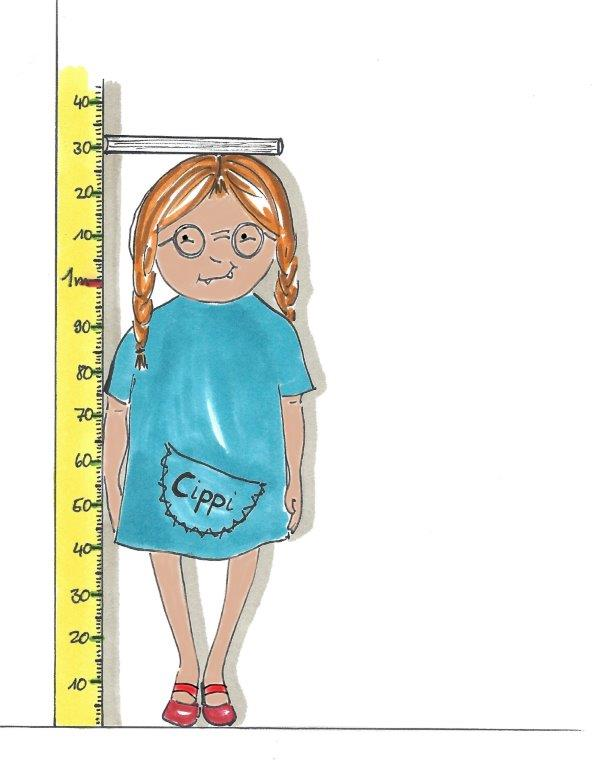
\includegraphics[width=0.6\textwidth]{content/3/chapter4/images/26.png}\\
Cippi量身高
\end{center}

三向比较操作符<=>通常称为宇宙飞船操作符。飞船操作符确定两个值A和B是A < B, A == B,还是A > B。开发者可以定义飞船操作符,或者使用编译器自动生成的。

为了理解三向比较运算符的优点,先从经典的运算方法开始。

\subsubsubsection{4.3.1\hspace{0.2cm}C++20前比较排序}

我使用MyInt简单的包装了int。这里,我想比较MyInt。下面是我使用的解决方案——函数模板isLessThan。

\hspace*{\fill} \\ %插入空行
\noindent
\textbf{MyInt支持的比较操作较少}
\begin{lstlisting}[style=styleCXX]
// comparisonOperator.cpp
#include <iostream>
struct MyInt {
	int value;
	explicit MyInt(int val): value{val} { }
	bool operator < (const MyInt& rhs) const {
		return value < rhs.value;
	}
};

template <typename T>
constexpr bool isLessThan(const T& lhs, const T& rhs) {
	return lhs < rhs;
}

int main() {
	std::cout << std::boolalpha << '\n';
	MyInt myInt2011(2011);
	MyInt myInt2014(2014);
	std::cout << "isLessThan(myInt2011, myInt2014): "
			  << isLessThan(myInt2011, myInt2014) << '\n';
	std::cout << '\n';
}
\end{lstlisting}

该程序按预期工作:

\begin{center}
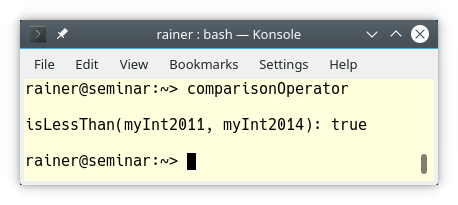
\includegraphics[width=0.6\textwidth]{content/3/chapter4/images/27.png}\\
使用小于运算符
\end{center}

老实说,MyInt是一个不直观的类型。当定义六个排序关系中的一个时,就应该定义所有的顺序关系。直观类型至少应该是半常规的。现在,我必须编写大量的样板代码。这是缺失的5个运算符。

\begin{lstlisting}[style=styleCXX]
bool operator == (const MyInt& rhs) const {
	return value == rhs.value;
}
bool operator != (const MyInt& rhs) const {
	return !(*this == rhs);
}
bool operator <= (const MyInt& rhs) const {
	return !(rhs < *this);
}
bool operator > (const MyInt& rhs) const {
	return rhs < *this;
}
bool operator >= (const MyInt& rhs) const {
	return !(*this < rhs);
}
\end{lstlisting}

现在,来看看C++20和三向比较运算符。

\subsubsubsection{4.3.2\hspace{0.2cm}C++20的顺序关系}

可以定义三向比较操作符,或者使用=default从编译器生成它。这两种情况下,可以自动得到所有六个比较运算符:==、!=、<、<=、>和>=。

\hspace*{\fill} \\ %插入空行
\noindent
\textbf{实现或生成的三向比较运算符}
\begin{lstlisting}[style=styleCXX]
// threeWayComparison.cpp

#include <compare>
#include <iostream>

struct MyInt {
	int value;
	explicit MyInt(int val): value{val} { }
	auto operator<=>(const MyInt& rhs) const {
		return value <=> rhs.value;
	}
};

struct MyDouble {
	double value;
	explicit constexpr MyDouble(double val): value{val} { }
	auto operator<=>(const MyDouble&) const = default;
};

template <typename T>
constexpr bool isLessThan(const T& lhs, const T& rhs) {
	return lhs < rhs;
}

int main() {

	std::cout << std::boolalpha << '\n';
	
	MyInt myInt1(2011);
	MyInt myInt2(2014);
	
	std::cout << "isLessThan(myInt1, myInt2): "
	          << isLessThan(myInt1, myInt2) << '\n';
	
	MyDouble myDouble1(2011);
	MyDouble myDouble2(2014);
	
	std::cout << "isLessThan(myDouble1, myDouble2): "
	          << isLessThan(myDouble1, myDouble2) << '\n';
	
	std::cout << '\n';

}
\end{lstlisting}

用户定义的(第9行)和编译器生成的(第17行)三向比较操作符如期工作。

\begin{center}
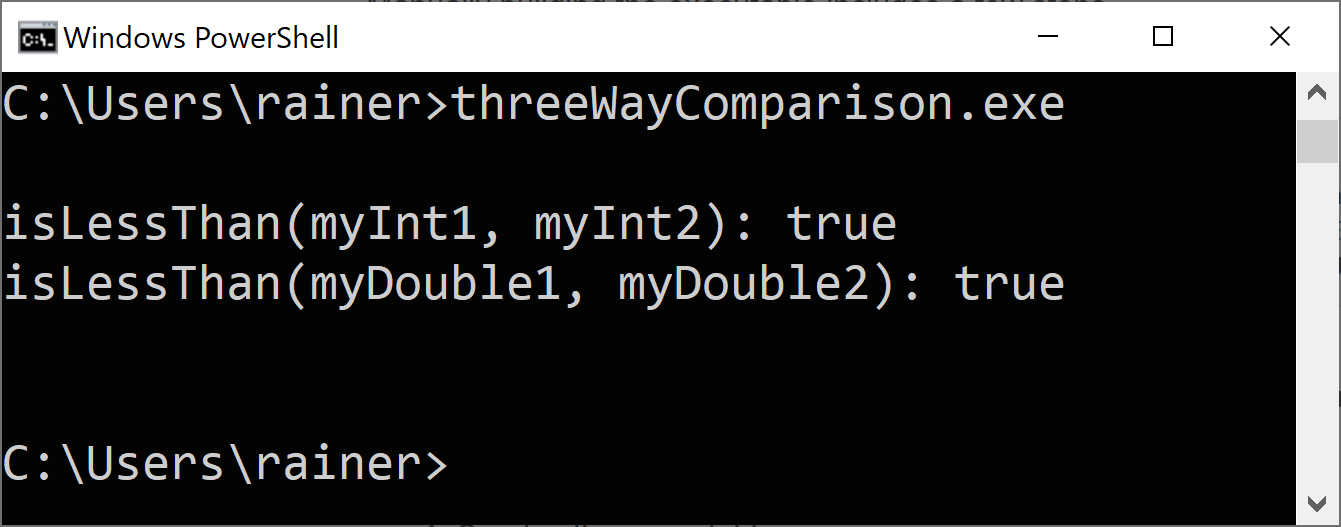
\includegraphics[width=0.6\textwidth]{content/3/chapter4/images/28.png}\\
\end{center}

在这种情况下,用户定义的和编译器生成的三向比较操作符之间有一些细微的区别。MyInt的编译器推导的返回类型(第9行)支持强排序,MyDouble的编译器推导的返回类型(第17行)支持部分排序。

\begin{tcolorbox}[breakable,enhanced jigsaw,colback=red!5!white,colframe=red!75!black,title={指针比较}]

编译器生成的三向比较运算符比较指针,但不比较引用的对象。

\begin{lstlisting}[style=styleCXX]
// spaceshipPoiner.cpp

#include <iostream>
#include <compare>
#include <vector>

struct A {
	std::vector<int>* pointerToVector;
	auto operator <=> (const A&) const = default;
};

int main() {

	std::cout << '\n';
	
	std::cout << std::boolalpha;
	
	A a1{new std::vector<int>()};
	A a2{new std::vector<int>()};
	
	std::cout << "(a1 == a2): " << (a1 == a2) << "\n\n";

}
\end{lstlisting}

令人惊讶的是,a1 == a2(第21行)的结果是false,而不是true,因为其比较了std::vector<int>*的地址。

\begin{tcblisting}{commandshell={}}
(a1 == a2): false
\end{tcblisting}

\end{tcolorbox}

并且,比较类别有三个。

\subsubsubsection{4.3.3\hspace{0.2cm}比较类别}

这三种比较类别的名称分别是强排序、弱排序和偏排序。对于T类型,以下三个属性区分三个比较类别。

\begin{enumerate}
\item 
T支持全部6种关系运算符:==、!=、<、<=、>和>=(简称:关系运算符)

\item 
所有相等的值都是一样的:(简称:等价)

\item 
T的所有值都具有可比性:对于T的任意值a和b, a < b、a == b和a > b三个关系中的一个必须为真(简称:可比性)
\end{enumerate}

当使用字符串的大小写不敏感表示作为排序标准时,等价值不必不同。此外,两个任意浮点值不需要具有可比性:对于a = 5.5, b = NaN(不是一个数字),以下表达式都不返回true: a < NaN, a == NaN,或a > NaN。

根据这三种性质,区分三种比较策略是很简单的:

\begin{table}[H]
\centering
\begin{tabular}{llll}
比较类别 & 关系操作符 & 等价 & 可比较 \\ \hline
强排序     & yes                 & yes         & yes        \\
弱排序       & yes                 &             & yes        \\
偏排序    & yes                 &             &           
\end{tabular}
\end{table}

支持强排序的类型支持隐式弱排序和部分排序,这同样适用于弱排序。支持弱排序的类型也支持部分排序。其他方向则不适用。

\begin{center}
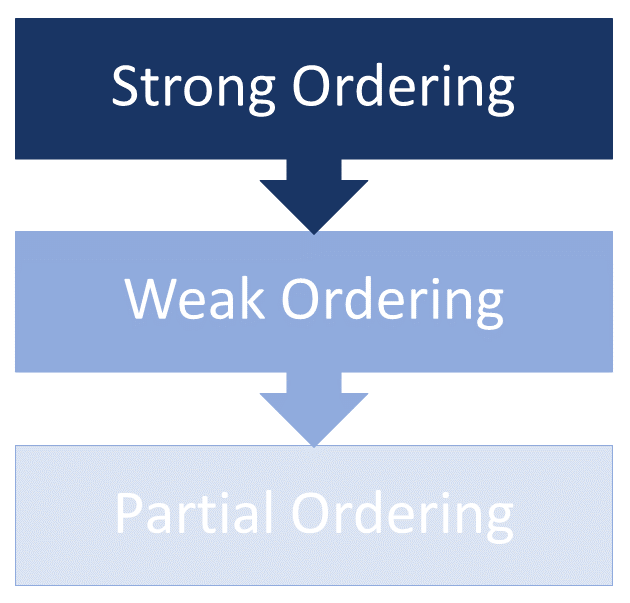
\includegraphics[width=0.4\textwidth]{content/3/chapter4/images/29.png}\\
强、弱、偏排序
\end{center}

若声明的返回类型是auto,则实际返回类型是基对象和成员子对象,以及要比较的成员数组元素的公共比较类别。

关于这条规则,先来看个例子:

\begin{lstlisting}[style=styleCXX]
// strongWeakPartial.cpp

#include <compare>

struct Strong {
	std::strong_ordering operator <=> (const Strong&) const = default;
};

struct Weak {
	std::weak_ordering operator <=> (const Weak&) const = default;
};

struct Partial {
	std::partial_ordering operator <=> (const Partial&) const = default;
};

struct StrongWeakPartial {

	Strong s;
	Weak w;
	Partial p;
	
	auto operator <=> (const StrongWeakPartial&) const = default;
	
	// FINE
	// std::partial_ordering operator <=> (const StrongWeakPartial&) const = default\
	;
	
	// ERROR
	// std::strong_ordering operator <=> (const StrongWeakPartial&) const = default;\
	
	// std::weak_ordering operator <=> (const StrongWeakPartial&) const = default; \


};

int main() {

	StrongWeakPartial a1, a2;
	
	a1 < a2;

}
\end{lstlisting}

类型StrongWeakPartial具有支持强(第6行)、弱(第10行)和偏排序(第14行)的子类型。因此,StrongWeakPartial类型(第17行)的常见比较类别是std::partial\_ordered。使用更强比较类别,例如强排序(第29行)或弱排序(第30行),将导致编译时错误。

现在,我想把重点放在编译器生成的宇宙飞船操作符上。

\subsubsubsection{4.3.4\hspace{0.2cm}编译器生成的宇宙飞船操作符}

编译器生成的三向比较运算符需要头文件<compare>,隐式地是constexpr和\href{https://www.modernescpp.com/index.php/c-core-guidelines-the-noexcept-specifier-and-operator}{noexcept},并执行字典顺序比较。

可以直接使用三向比较运算符。

\hspace*{\fill} \\ %插入空行
\noindent
\textbf{4.3.4.1\hspace{0.2cm}直接使用三向比较运算符}

spaceship.cpp直接使用太空船操作符。

\begin{lstlisting}[style=styleCXX]
// spaceship.cpp

#include <compare>
#include <iostream>
#include <string>
#include <vector>

int main() {
	
	std::cout << '\n';
	
	int a(2011);
	int b(2014);
	auto res = a <=> b;
	if (res < 0) std::cout << "a < b" << '\n';
	else if (res == 0) std::cout << "a == b" << '\n';
	else if (res > 0) std::cout << "a > b" << '\n';
	
	std::string str1("2014");
	std::string str2("2011");
	auto res2 = str1 <=> str2;
	if (res2 < 0) std::cout << "str1 < str2" << '\n';
	else if (res2 == 0) std::cout << "str1 == str2" << '\n';
	else if (res2 > 0) std::cout << "str1 > str2" << '\n';
	
	std::vector<int> vec1{1, 2, 3};
	std::vector<int> vec2{1, 2, 3};
	auto res3 = vec1 <=> vec2;
	if (res3 < 0) std::cout << "vec1 < vec2" << '\n';
	else if (res3 == 0) std::cout << "vec1 == vec2" << '\n';
	else if (res3 > 0) std::cout << "vec1 > vec2" << '\n';
	
	std::cout << '\n';

}
\end{lstlisting}

程序对int(第14行)、string(第21行)和vector(第28行)使用了太空船操作符。下面是程序的输出。

\begin{tcblisting}{commandshell={}}
a < b
str1 > str2
vec1 == vec2
\end{tcblisting}

如前所述,这些比较是constexpr,可以在编译时完成。

\hspace*{\fill} \\ %插入空行
\noindent
\textbf{4.3.4.2\hspace{0.2cm}编译时的比较}

三向比较操作符是隐式的constexpr。因此,可以简化前面的程序threewaycompare.cpp,并在编译时比较下面程序中的MyDouble。

\begin{lstlisting}[style=styleCXX]
// threeWayComparisonAtCompileTime.cpp

#include <compare>
 #include <iostream>

struct MyDouble {
	 double value;
	 explicit constexpr MyDouble(double val): value{val} { }
	 auto operator<=>(const MyDouble&) const = default;
};

 template <typename T>
 constexpr bool isLessThan(const T& lhs, const T& rhs) {
	 return lhs < rhs;
}

 int main() {
	
	std::cout << std::boolalpha << '\n';
	
	constexpr MyDouble myDouble1(2011);
	constexpr MyDouble myDouble2(2014);
	
	constexpr bool res = isLessThan(myDouble1, myDouble2);
	
	std::cout << "isLessThan(myDouble1, myDouble2): "
	<< res << '\n';
	
	std::cout << '\n';

}
\end{lstlisting}

在编译时进行比较(第24行),并得到了比较结果。

\begin{center}
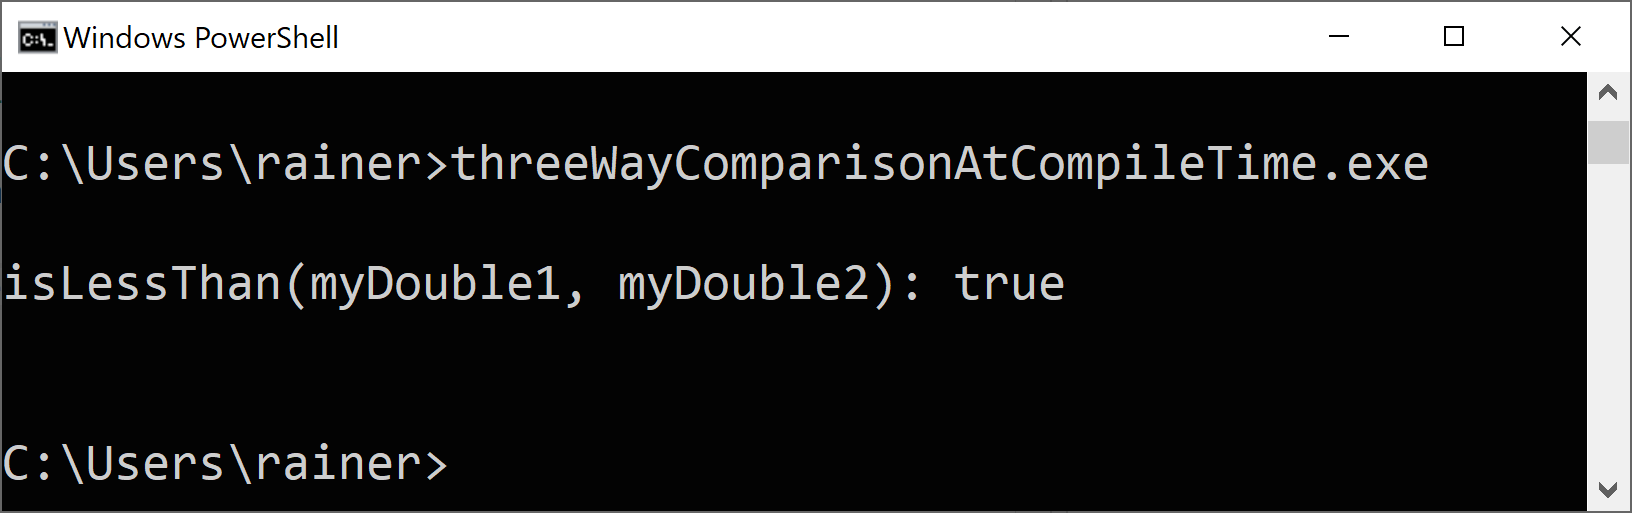
\includegraphics[width=0.6\textwidth]{content/3/chapter4/images/30.png}\\
使用constexpr编译器生成的太空船操作符
\end{center}

\hspace*{\fill} \\ %插入空行
\noindent
\textbf{4.3.4.3\hspace{0.2cm}直接使用三向比较运算符}

编译器生成的三向比较运算符执行字典顺序比较。本例中,字典比较意味着从左到右比较所有基类,以及类的所有非静态成员的声明顺序。所以,必须加以限定:出于性能原因,编译器生成的==和!=运算符在C++20中的表现不同。我将在优化的==和!=操作符一节中再来详谈。

来自Microsoft C++团队博客的帖子\href{https://devblogs.microsoft.com/cppblog/simplify-your-code-with-rocket-science-c20s-spaceship-operator/}{“用火箭科学简化代码:C++20的宇宙飞船操作符”}提供了一个令人印象深刻的字典比较例子。为了可读性,我添加了一些注释。

\hspace*{\fill} \\ %插入空行
\noindent
\textbf{字典序的比较}
\begin{lstlisting}[style=styleCXX]
struct Basics {
	 int i;
	 char c;
	 float f;
	 double d;
	 auto operator<=>(const Basics&) const = default;
};

struct Arrays {
	 int ai[1];
	 char ac[2];
	 float af[3];
	 double ad[2][2];
	 auto operator<=>(const Arrays&) const = default;
};

 struct Bases : Basics, Arrays {
	 auto operator<=>(const Bases&) const = default;
};

int main() {
	constexpr Bases a = { { 0, 'c', 1.f, 1. }, // Basics
	 					{ { 1 }, { 'a', 'b' }, { 1.f, 2.f, 3.f }, // Arrays
						{ { 1., 2. }, { 3., 4. } } } };
	constexpr Bases b = { { 0, 'c', 1.f, 1. }, // Basics
	 					{ { 1 }, { 'a', 'b' }, { 1.f, 2.f, 3.f }, // Arrays
		 				{ { 1., 2. }, { 3., 4. } } } };
	static_assert(a == b);
	static_assert(!(a != b));
	static_assert(!(a < b));
	static_assert(a <= b);
	static_assert(!(a > b));
	static_assert(a >= b);
}
\end{lstlisting}

我认为这个程序最具挑战性的方面不是宇宙飞船操作符,而是通过聚合初始化来初始化Bases(第22和25行)。当成员都是public时,聚合初始化使我们能够直接初始化类类型(class、struct、union)的成员,所以可以使用大括号初始化。聚合初始化将在C++20中指定初始化器一节中更详细地讨论。

\begin{tcolorbox}[breakable,enhanced jigsaw,colback=blue!5!white,colframe=blue!75!black,title={优化的==和!=操作符}]

对于类似字符串或类vector类型,存在优化潜力。这种情况下,==和!=可能比编译器生成的三向比较运算符更快。若比较的两个值的长度不同,==和!=操作符可以停止。否则,若一个值是另一个值的前缀,则将比较所有元素,直到较短的值结束为止。标准化委员会意识到了这个性能问题,并通过论文\href{http://www.open-std.org/jtc1/sc22/wg21/docs/papers/2019/p1185r2.html}{P1185R2}解决了这个问题。因此,编译器生成的==和!=操作符(对于类字符串或类vector类型)首先会比较其长度,必要时再比较其内容。

\end{tcolorbox}

现在,是时候介绍C++中的一些新东西了。C++20引入了重写表达式的概念。

\subsubsubsection{4.3.5\hspace{0.2cm}重写表达式}

当编译器看到诸如a < b之类的东西时,会使用太空船操作符将其重写为(a <=> b) < 0。

当然,该规则适用于所有六个比较运算符:a OP b变成(a <=> b) OP 0。这就更好了。若没有类型(a)到类型(b)的转换,编译器生成新的表达式为0 OP (b <=> a)。

例如,对于小于操作符,若(a <=> b) < 0不起作用,编译器会生成0 < (b <=> a)。本质上,编译器负责比较操作符的对称性。

下面是一些重写表达式的例子:

\hspace*{\fill} \\ %插入空行
\noindent
\textbf{使用重写表达式的MyInt}
\begin{lstlisting}[style=styleCXX]
// rewritingExpressions.cpp

#include <compare>
#include <iostream>

class MyInt {
public:
	 constexpr MyInt(int val): value{val} { }
	 auto operator<=>(const MyInt& rhs) const = default;
private:
	 int value;
};

int main() {
	
	std::cout << '\n';
	
	constexpr MyInt myInt2011(2011);
	constexpr MyInt myInt2014(2014);
	
	constexpr int int2011(2011);
	constexpr int int2014(2014);
	
	if (myInt2011 < myInt2014) std::cout << "myInt2011 < myInt2014" << '\n';
	if ((myInt2011 <=> myInt2014) < 0) std::cout << "myInt2011 < myInt2014" << '\n';
	
	std::cout << '\n';
	
	if (myInt2011 < int2014) std:: cout << "myInt2011 < int2014" << '\n';
	if ((myInt2011 <=> int2014) < 0) std:: cout << "myInt2011 < int2014" << '\n';
	
	std::cout << '\n';
	
	if (int2011 < myInt2014) std::cout << "int2011 < myInt2014" << '\n';
	if (0 < (myInt2014 <=> int2011)) std:: cout << "int2011 < myInt2014" << '\n';
	
	std::cout << '\n';

}
\end{lstlisting}

第24行、第29行和第34行中使用了小于操作符和相应的太空船表达式。第35行是最有趣的。它举例说明了比较(int2011 < myInt2014)如何触发飞船表达式(0 < (myInt2014 <=> int2011)的生成。

\begin{tcblisting}{commandshell={}}
myInt2011 < myInt2014
myInt2011 < myInt2014

myInt2011 < int2014
myInt2011 < int2014

int2011 < myInt2014
int2011 < myInt2014
\end{tcblisting}

老实说,MyInt有一个问题:构造函数接受一个参数应该声明为explicit。接受一个参数的构造函数,如MyInt(int val)(第8行)是转换构造函数。所以MyInt的实例可以由任意整数或浮点值生成,因为每个整数或浮点值都可以隐式地转换为int。

来修复这个问题,并使构造函数MyInt(int val)为显式。为了支持MyInt和int的比较,MyInt需要用于int的三向比较操作符。

\hspace*{\fill} \\ %插入空行
\noindent
\textbf{int的另一个三向比较运算符}
\begin{lstlisting}[style=styleCXX]
// threeWayComparisonForInt.cpp

#include <compare>
#include <iostream>

class MyInt {
public:
	constexpr explicit MyInt(int val): value{val} { }
	
	auto operator<=>(const MyInt& rhs) const = default;
	
	constexpr auto operator<=>(const int& rhs) const {
		return value <=> rhs;
	}
private:
	int value;
};

template <typename T, typename T2>
constexpr bool isLessThan(const T& lhs, const T2& rhs) {
	return lhs < rhs;
}

int main() {

	std::cout << std::boolalpha << '\n';
	
	constexpr MyInt myInt2011(2011);
	constexpr MyInt myInt2014(2014);
	
	constexpr int int2011(2011);
	constexpr int int2014(2014);
	
	std::cout << "isLessThan(myInt2011, myInt2014): "
	<< isLessThan(myInt2011, myInt2014) << '\n';
	
	std::cout << "isLessThan(int2011, myInt2014): "
	<< isLessThan(int2011, myInt2014) << '\n';
	
	std::cout << "isLessThan(myInt2011, int2014): "
	<< isLessThan(myInt2011, int2014) << '\n';
	
	constexpr auto res = isLessThan(myInt2011, int2014);
	
	std::cout << '\n';

}
\end{lstlisting}

我在(第10行)中定义了三向比较运算符,并将其声明为constexpr。用户定义的三向比较操作符不是隐式的constexpr,这与编译器生成的三向比较操作符不同。在每个组合中都可以比较MyInt和int(第34、37和40行)。

\begin{tcblisting}{commandshell={}}
isLessThan(MyInt2011, myInt2014): true
isLessThan(int2011, myInt2014): true
isLessThan(MyInt2011, int2014): true
\end{tcblisting}

老实说,各种三向比较运算符的实现非常优雅。编译器自动生成MyInt的比较,并且用户显式地定义了与int的比较。此外,由于重新排序,需定义2个操作符就可以得到18 = 3 * 6个比较操作符的组合。3代表int OP MyInt, MyInt OP MyInt和MyInt OP int的组合,6代表六个比较运算符。

\subsubsubsection{4.3.6\hspace{0.2cm}用户定义和自动生成的比较操作符}

可以定义六个比较操作符中的一个,并使用太空船操作符自动生成所有比较操作符时,有一个问题:哪个具有更高的优先级?例如,MyInt有一个用户定义的小于等于运算符,还有编译器生成的6个比较运算符。

看看会发生什么。

\hspace*{\fill} \\ %插入空行
\noindent
\textbf{用户定义的操作符和自动生成的操作符间的互动}
\begin{lstlisting}[style=styleCXX]
// userDefinedAutoGeneratedOperators.cpp

#include <compare>
#include <iostream>

class MyInt {
public:
	constexpr explicit MyInt(int val): value{val} { }
	bool operator == (const MyInt& rhs) const {
	std::cout << "== " << '\n';
		return value == rhs.value;
	}
	bool operator < (const MyInt& rhs) const {
	std::cout << "< " << '\n';
		return value < rhs.value;
	}
	
	auto operator<=>(const MyInt& rhs) const = default;

private:
	int value;
};

int main() {

	MyInt myInt2011(2011);
	MyInt myInt2014(2014);
	
	myInt2011 == myInt2014;
	myInt2011 != myInt2014;
	myInt2011 < myInt2014;
	myInt2011 <= myInt2014;
	myInt2011 > myInt2014;
	myInt2011 >= myInt2014;

}
\end{lstlisting}

为了查看用户定义的==和<操作符的作用,我将相应的消息写入std::cout。因为std::cout是一个运行时操作,所以这两个操作符都不能是constexpr。

看看会发生什么:

\begin{tcblisting}{commandshell={}}
==
==
<
\end{tcblisting}

编译器使用用户定义的==(第29和30行)和<操作符(第31行)。此外,编译器使用==运算符生成了!=运算符(第30行)。另一方面,编译器不会使用!=操作符生成==操作符。

\begin{tcolorbox}[breakable,enhanced jigsaw,colback=blue!5!white,colframe=blue!75!black,title={与Python的相似性}]
Python 3中,编译器在必要时从==中生成!=,而不是反过来。在Python 2中,所谓的富比较(用户自定义的六个比较操作符)的优先级高于Python的三向比较操作符\_\_cmp\_\_。相似度高的那个,我看得是Python 2,因为三向比较运算符\_\_cmp\_\_在Python 3中删除了。
\end{tcolorbox}	

\begin{tcolorbox}[breakable,enhanced jigsaw,colback=mygreen!5!white,colframe=mygreen!75!black,title={总结}]
\begin{itemize}
\item 
通过默认操作符<=>,编译器自动生成6个比较操作符。编译器生成的比较运算符应用字典顺序的比较:所有基类从左到右比较,类的所有非静态成员按声明顺序比较。

\item 
当自动生成的比较操作符和用户定义的比较操作符同时存在时,用户定义的比较操作符具有更高的优先级。

\item 
编译器重写表达式以保证比较操作符的对称性。例如,若(a <=> b) < 0不起作用,则编译器会生成0 < (b <=> a)。
\end{itemize}
\end{tcolorbox}	
























